\documentclass{article}
\usepackage[utf8]{inputenc}

%meer ams meer beter
\usepackage{amsmath}
\usepackage{amssymb}
\usepackage{amsthm} %nodig voor blokje

\usepackage{marginnote}
\usepackage[margin=1in,footskip=0.25in]{geometry} %heb wat meer ruimte

%Plaatjes
\usepackage{graphicx}
\usepackage{float}
\usepackage{caption}
\usepackage{subcaption}
\usepackage{epstopdf}

\begin{document}
\begin{figure}[h]
\centering

<<<<<<< HEAD
\includegraphics{QQplotY1sw.eps}
=======
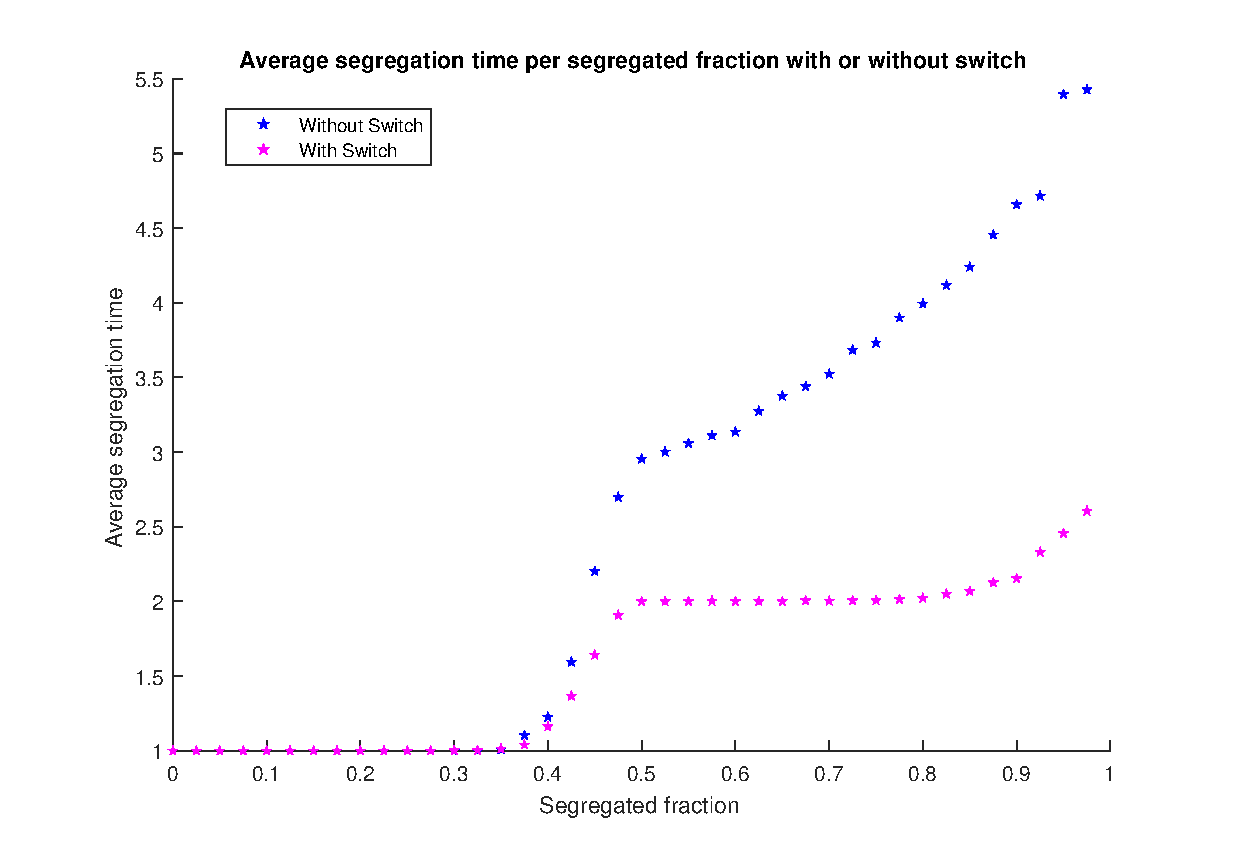
\includegraphics{Avesegsw2.eps}
>>>>>>> 0e99d952b1a7b39cc9186a01f5264941ecc361eb
\caption{a nice plot}
\label{fig:mesh1}
\end{figure}
\end{document}